\documentclass{beamer}

%\usepackage{pgfpages}
%\setbeameroption{show notes on second screen=right}

%DEFAULT
\usepackage[utf8]{inputenc}
\usepackage[german]{babel}
\usepackage[T1]{fontenc}
\usepackage{mathtools}
\usepackage{amsmath}
\usepackage{amsfonts}
\usepackage{amssymb}

%theming
%\usetheme{Montpellier}
%\setbeamertemplate{note page}{\pagecolor{yellow!5}\insertnote}

%GRAPHING
\usepackage{tikz-network}
\usepackage{adjustbox}
\usepackage{subcaption}

%BIBTEX
\usepackage[numbers,square]{natbib}

%META-INFORMATION
\author{Maximilian Moeller}
\title{Maximaler Fluss in Flussnetzwerken}
\date{\today}

%ALIAS
\newcommand{\ff}{Ford-Fulkerson}
\newcommand{\pr}{Push/Relabel}

\begin{document}
\begin{frame}
\maketitle
\center\large Proseminar Theoretische Informatik 2020
\end{frame}

\begin{frame}
\frametitle{Gliederung}
\tableofcontents
\note{Beweise nicht ausgeführt, nur Beweisideen}
alle Codesnippets und Definitionen aus \citep{Cormen09}
\end{frame}

\section{Motivation}
\begin{frame}
\frametitle{Motivation}
\begin{columns}
\begin{column}{.4\textwidth}
\begin{itemize}
\item (Stoff-) Mengen auf mehreren Pfaden gleichzeitig transportiert
\item Pfade durch Kapazitäten beschränkt\pause
\item Beispiel Rechnernetze: Maximale Anzahl der gleichzeitig transportierten Pakete von A nach B?
\end{itemize}
\note{!= Kapazitätsproblem}
\note{Alle Definitionen etc. aus \citep{Cormen09}}
\end{column}
\begin{column}{.6\textwidth}
\begin{tikzpicture}
\Vertex[label=$A$]{s}
\Vertex[label=$S1$, x=2, y=1]{1}
\Vertex[label=$S2$, x=2, y=-1]{2}
\Vertex[label=$S3$, x=4, y=1]{3}
\Vertex[label=$S4$, x=4, y=-1]{4}
\Vertex[label=$B$, x=6, y=0]{t}
\Edge[Direct, label=4](s)(1)
\Edge[Direct, label=7](s)(2)
\Edge[Direct, label=2](1)(3)
\Edge[Direct, label=4](2)(3)
\Edge[Direct, label=3](2)(4)
\Edge[Direct, label=6](3)(t)
\Edge[Direct, label=2](4)(t)
\end{tikzpicture}
\note{Kapazitäten = Bandbreite d. Kanals}
\note{maximal 8 Pakete}
\end{column}
\end{columns}
\end{frame}


\section{Grundlagen}
\subsection{Flussnetzwerke}
\begin{frame}
\frametitle{Flussnetzwerke}
\begin{columns}
\begin{column}{.45\textwidth}
\begin{itemize}
\item gerichteter Graph $G=(V,E)$
\item Kapazitäten $c: E \to \mathbb{N}$\\$\forall (u,v)\in E: c(u,v) \geq 0$
\item Quelle $s$ und Senke $t$
\item Pfade für alle Knoten\\$\forall v \in V:s \to v \to t$
\item Keine reflexiven Kanten\\$\forall v \in V: (v,v)\not\in E$
\end{itemize}
\note{reflexive Kanten verboten: Beispiel Spannung beim Stromfluss}
\end{column}
\begin{column}{.6\textwidth}
\begin{adjustbox}{width=\textwidth}
\begin{tikzpicture}
\Vertex[label=$s$]{s}
\Vertex[label=$v_1$, x=2, y=1]{1}
\Vertex[label=$v_2$, x=2, y=-1]{2}
\Vertex[label=$v_3$, x=4, y=1]{3}
\Vertex[label=$v_4$, x=4, y=-1]{4}
\Vertex[label=$t$, x=6, y=0]{t}
\Edge[Direct, label=4](s)(1)
\Edge[Direct, label=7](s)(2)
\Edge[Direct, label=2](1)(3)
\Edge[Direct, label=4](2)(3)
\Edge[Direct, label=3](2)(4)
\Edge[Direct, label=6](3)(t)
\Edge[Direct, label=2](4)(t)
\end{tikzpicture}
\end{adjustbox}
\end{column}
\end{columns}
\end{frame}

\begin{frame}
\frametitle{unzulässige Spezialfälle}
\note{aus algorithmischen Gründen (Restnetzwerke)}
\begin{figure}
\begin{adjustbox}{width=0.45\linewidth}
\begin{tikzpicture}
\Vertex[label=$s$]{s}
\Vertex[label=$v_1$, x=1.5, y=1]{1}
\Vertex[label=$v_2$, x=1.5, y=-1]{2}
\Vertex[label=$t$, x=3, y=0]{t}
\Edge[Direct, label=4](s)(1)
\Edge[Direct, label=7](s)(2)
\Edge[Direct, label=2, bend=15](1)(2)
\Edge[Direct, label=4,bend=15](2)(1)
\Edge[Direct, label=3](1)(t)
\Edge[Direct, label=6](2)(t)
\end{tikzpicture}
\end{adjustbox}
\pause
\hfill
\begin{adjustbox}{width=0.45\linewidth}
\begin{tikzpicture}
\Vertex[label=$s$]{s}
\Vertex[label=$v_1$, x=1.5, y=1]{1}
\Vertex[label=$v_2$, x=1.5, y=-1]{2}
\Vertex[label=$v_{12}$, x= 2, y=0]{3}
\Vertex[label=$t$, x=3, y=0]{t}
\Edge[Direct, label=4](s)(1)
\Edge[Direct, label=7](s)(2)
\Edge[Direct, label=2](1)(3)
\Edge[Direct, label=2](3)(2)
\Edge[Direct, label=4,bend=15](2)(1)
\Edge[Direct, label=3](1)(t)
\Edge[Direct, label=6](2)(t)
\end{tikzpicture}
\end{adjustbox}
\caption{Modellierung von antiparallelen Kanten durch zusätzliche Knoten}
\end{figure}
\end{frame}

\begin{frame}
\frametitle{unzulässige Spezialfälle}
\note{nicht schwerer als mit einer Quelle/Senke}
\begin{figure}
\begin{adjustbox}{width=0.45\linewidth}
\begin{tikzpicture}
\Vertex[x=-1, Pseudo]{p1}
\Vertex[label=$s1$, y=2]{s1}
\Vertex[label=$s2$, y=0]{s2}
\Vertex[label=$s3$, y=-2]{s3}
\Vertex[label=$v$, x=1, y=0]{1}
\Vertex[label=$t1$, x=2, y=1]{t1}
\Vertex[label=$t2$, x=2, y=-1]{t2}
\Vertex[x=3, Pseudo]{p2}
\Edge[Direct, label=4](s1)(1)
\Edge[Direct, label=7](s2)(1)
\Edge[Direct, label=2](s3)(1)
\Edge[Direct, label=4](1)(t1)
\Edge[Direct, label=3](1)(t2)
\end{tikzpicture}
\end{adjustbox}
\pause
\hfill
\begin{adjustbox}{width=0.45\linewidth}
\begin{tikzpicture}
\Vertex[label=$s$, x=-1]{s}
\Vertex[label=$s1$, y=2]{s1}
\Vertex[label=$s2$, y=0]{s2}
\Vertex[label=$s3$, y=-2]{s3}
\Vertex[label=$v$, x=1, y=0]{1}
\Vertex[label=$t1$, x=2, y=1]{t1}
\Vertex[label=$t2$, x=2, y=-1]{t2}
\Vertex[label=$t$, x=3]{t}
\Edge[Direct, label=$\infty$](s)(s1)
\Edge[Direct, label=$\infty$](s)(s2)
\Edge[Direct, label=$\infty$](s)(s3)
\Edge[Direct, label=4](s1)(1)
\Edge[Direct, label=7](s2)(1)
\Edge[Direct, label=2](s3)(1)
\Edge[Direct, label=4](1)(t1)
\Edge[Direct, label=3](1)(t2)
\Edge[Direct, label=$\infty$](t1)(t)
\Edge[Direct, label=$\infty$](t2)(t)
\end{tikzpicture}
\end{adjustbox}
\caption{Modellierung von mehreren Quellen und Senken durch Superquelle und Supersenke}
\end{figure}
\end{frame}

\subsection{Fluss}
\begin{frame}
\frametitle{Fluss in Flussnetzwerken}
\begin{itemize}
\item Fluss $f: V \times V \to \mathbb{N}$
\item erfüllt drei Bedingungen:
\begin{equation}
\forall u,v\in V\colon (u,v)\notin E\Rightarrow f(u,v) = 0
\end{equation}
\begin{equation}
\forall u,v\in V\colon 0\leq f(u,v)\leq c(u,v)
\end{equation}
\begin{equation}
\forall u\in V\setminus\{s,t\}\colon\sum_{v\in V} f(v,u) = \sum_{v\in V} f(u,v)
\end{equation}
\note{Flusserhaltung, entspricht Kirchhoffscher Knotenregel}
\end{itemize}
\end{frame}

\begin{frame}
\frametitle{Notation}
\begin{columns}
\begin{column}{.4\textwidth}
\begin{itemize}
\item $f(u,v)/c(u,v)$
\note{bei $f(u,v) = 0$ wird nur $c(u,v)$ angegeben}
\end{itemize}
\end{column}
\begin{column}{.55\textwidth}
\begin{adjustbox}{width=\textwidth}
\begin{tikzpicture}
\Vertex[label=$s$]{s}
\Vertex[label=$v_1$, x=2, y=1]{1}
\Vertex[label=$v_2$, x=2, y=-1]{2}
\Vertex[label=$v_3$, x=4, y=1]{3}
\Vertex[label=$v_4$, x=4, y=-1]{4}
\Vertex[label=$t$, x=6, y=0]{t}
\Edge[Direct, label=1/4](s)(1)
\Edge[Direct, label=2/7](s)(2)
\Edge[Direct, label=1/2](1)(3)
\Edge[Direct, label=4](2)(3)
\Edge[Direct, label=2/3](2)(4)
\Edge[Direct, label=1/6](3)(t)
\Edge[Direct, label=2/2](4)(t)
\end{tikzpicture}
\end{adjustbox}
\end{column}
\end{columns}
\end{frame}

\begin{frame}
\frametitle{Wert eines Flusses}
\begin{columns}
\begin{column}{.45\textwidth}
Wert $\lvert f \rvert$ eines Flusses $f$:
\begin{equation}
\lvert f \rvert = \sum_{u\in V} f(s,u) - \sum_{u\in V} f(u,s) \nonumber
\end{equation}
\note{Meist nur linker Term.}
\note{"Netto"}
\note{wegen Flusserhaltung gleich zu eingehendem Fluss in Senke}
\end{column}
\hfill
\pause
\begin{column}{.45\textwidth}
\begin{figure}
\begin{adjustbox}{width=\textwidth}
\begin{tikzpicture}
\Vertex[label=$s$]{s}
\Vertex[label=$u_1$, x=2, y=1]{1}
\Vertex[label=$u_2$, x=2, y=-1]{2}
\Vertex[label=$u_3$, x=4, y=1]{3}
\Vertex[label=$u_4$, x=4, y=-1]{4}
\Vertex[label=$t$, x=6, y=0]{t}
\Edge[Direct, label=2/4](s)(1)
\Edge[Direct, label=6/7](s)(2)
\Edge[Direct, label=2/2](1)(3)
\Edge[Direct, label=4/4](2)(3)
\Edge[Direct, label=2/3](2)(4)
\Edge[Direct, label=6/6](3)(t)
\Edge[Direct, label=2/2](4)(t)
\end{tikzpicture}
\end{adjustbox}
\caption{Ein Fluss $f_{max}$ mit $\lvert f_{max} \rvert = 8$}
\end{figure}
\end{column}
\end{columns}
\end{frame}

\begin{frame}
\frametitle{Maximaler-Fluss-Problem}
\begin{flushleft}
Gegeben: ein Flussnetzwerk $G = (V,E)$ und dessen Kapazitätsfunktion $c: V \times V \to \mathbb{N}$.\linebreak
Gesucht: ein Fluss $f$, dessen Wert $\lvert f \rvert$ maximal für dieses Flussnetzwerk ist.
\end{flushleft}
\end{frame}

\section{weitere Theorie}
\subsection{Restnetzwerke}
\begin{frame}
\frametitle{Restnetzwerke}
\begin{itemize}
\item Fluss $f$ in Flussnetzwerk $G=(V,E)$ induziert Restnetzwerk $G_{f}=(V,E_{f})$
\item mit $E_f = \{ (u,v) \in V \times V \mid c_{f}(u,v) > 0\}$
\item wobei für $u,v \in V$ gilt: 
\end{itemize}
\begin{equation}
c_{f}(u,v) = 
\begin{cases}
c(u,v) - f(u,v) & \text{falls $(u,v)\in E$}\\
f(v,u) & \text{falls $(v,u) \in E$}\\
0 & \text{sonst}
\end{cases}
\nonumber
\end{equation}
\note{antiparallele Kanten möglich -> kein Flussnetzwerk}
\note{Überleitung Beispiele}
\end{frame}

\begin{frame}
\frametitle{Restnetzwerke}
\begin{figure}[T]
\centering
\begin{subfigure}{0.45\textwidth}
\begin{adjustbox}{width =\linewidth}
\begin{tikzpicture}
\Vertex[label=$s$, x=1]{s}
\Vertex[label=$v_1$, x=2.25, y=1]{1}
\Vertex[label=$v_2$, x=2.25, y=-1]{2}
\Vertex[label=$v_3$, x=3.75, y=1]{3}
\Vertex[label=$v_4$, x=3.75, y=-1]{4}
\Vertex[label=$t$, x=5, y=0]{t}
\Edge[Direct, label=1/4](s)(1)
\Edge[Direct, label=2/7](s)(2)
\Edge[Direct, label=1/2](1)(3)
\Edge[Direct, label=4](2)(3)
\Edge[Direct, label=2/3](2)(4)
\Edge[Direct, label=1/6](3)(t)
\Edge[Direct, label=2/2](4)(t)
\end{tikzpicture}
\end{adjustbox}
\caption{Fluss $f$ in einem Flussnetzwerk $G = (V,E)$}
\end{subfigure}
\hfill
\begin{subfigure}{0.45\textwidth}
\begin{adjustbox}{width =\linewidth}
\begin{tikzpicture}
\Vertex[label=$s$, x=1]{s}
\Vertex[label=$v_1$, x=2.25, y=1]{1}
\Vertex[label=$v_2$, x=2.25, y=-1]{2}
\Vertex[label=$v_3$, x=3.75, y=1]{3}
\Vertex[label=$v_4$, x=3.75, y=-1]{4}
\Vertex[label=$t$, x=5, y=0]{t}
\Edge[Direct, label=3, bend=15](s)(1)
\Edge[Direct, label=1, bend=15](1)(s)
\Edge[Direct, label=5, bend=15](s)(2)
\Edge[Direct, label=2, bend=15](2)(s)
\Edge[Direct, label=1, bend=15](1)(3)
\Edge[Direct, label=1, bend=15](3)(1)
\Edge[Direct, label=4](2)(3)
\Edge[Direct, label=1, bend=15](2)(4)
\Edge[Direct, label=2, bend=15](4)(2)
\Edge[Direct, label=5, bend=15](3)(t)
\Edge[Direct, label=1, bend=15](t)(3)
\Edge[Direct, label=2](t)(4)
\end{tikzpicture}
\end{adjustbox}
\caption{Restnetzwerk $G_f = (V,E_f)$}
\end{subfigure}
\end{figure}
\note{Kanten in ursprünglicher Flussrichtung: wie viel mehr Fluss noch zulässig}
\note{Kanten entgegen Flussrichtung: wie viel Fluss kann zurückgeschickt werden}
\note{Kanten mit Restkapazität 0 nicht eingezeichnet}
\begin{itemize}
\item Definition eines Flusses $f'$ im Restnetzwerk analog zu Fluss in Flussnetzwerken.
\end{itemize}
\end{frame}

\begin{frame}
\frametitle{Erhöhung eines Flusses}
\begin{itemize}
\item Flussnetzwerk $G=(V,E)$ mit Fluss $f$
\item Restnetzwerk $G_f$ mit Fluss $f'$
\end{itemize}
\vspace{0.05\textheight}
\begin{align*}
(f \uparrow f')(u,v)&=
\begin{cases}
f(u,v) + f'(u,v) - f'(v,u) & \text{falls $(u,v) \in E$}\\
0 & \text{sonst}
\end{cases}\\
\lvert f\uparrow f' \rvert &= \lvert f \rvert + \lvert f'\rvert
\end{align*}
\note{$f \uparrow f'$ erklären}
\vspace{0.05\textheight}
Beweis über Umformen der Summen.
\note{Jetzt noch zu tun: finden eines Flusses in Gf -> Erweiterungspfade}
\end{frame}

\subsection{Erweiterungspfade}
\begin{frame}
\frametitle{Erweiterungspfade}
\begin{itemize}
\item Pfad $p$ im Restnetzwerk $G_f$ von $s$ nach $t$
\item Pfadkapazität $c_f(p) = min\{ c_f(u,v)\mid (u,v) \text{ liegt auf $p$}\}$
\item Definiere Fluss $f_p$ entlang von $p$ mit $f_p(u,v) = \begin{cases}c_f(p) & \text{falls $(u,v)$ auf $p$ liegt}\\0 & \text{sonst}\end{cases}$
\item dann: $\lvert f\uparrow f_p \rvert = \lvert f \rvert + \lvert f_p\rvert > \lvert f\rvert$
\end{itemize}
\note{alles zusammen für \ff-Algorithmus}
\end{frame}

\section{Algorithmen}
\subsection{Ford-Fulkerson}
\begin{frame}
\frametitle{\ff-Basisalgorithmus}
\begin{adjustbox}{width = \textwidth}
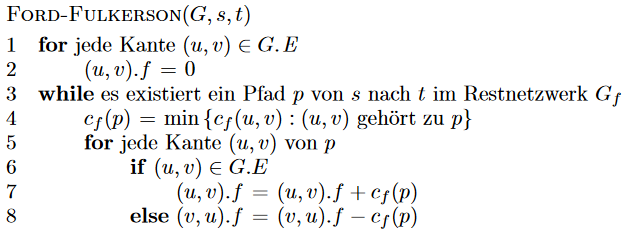
\includegraphics{../Grafiken/FF-Basis.png}
\end{adjustbox}
\note{Jack Edmonds und Richard Karp, 1970}
\end{frame}

\begin{frame}
\frametitle{\ff-Basisalgorithmus}
\begin{itemize}
\item Fluss ist maximal wegen maxflow-mincut-Theorem \begin{itemize}
\item u.A.: $\lvert f\rvert$ ist maximal $\Leftrightarrow$ kein Erweiterungspfad in $G_{f}$
\end{itemize}
\item Terminiert stets bei Kantengewichten aus $\mathbb{N}$
\item $\mathcal{O}(\lvert f_{max}\rvert \cdot E)$ für einen maximalen Fluss $f_{max}$
\item Problem: schlechte Wegewahl möglich
\end{itemize}
\note{bei rationalen Zahlen Multiplikation mit Hauptnenner}
\note{Terminierung bzw. Konvergenz bei reellen Zahlen nicht sichergestellt}
\end{frame}

\begin{frame}
\frametitle{schlechte Wegewahl}
\begin{figure}[T]
\centering
\begin{subfigure}{0.45\textwidth}
\begin{adjustbox}{width =\linewidth}
\begin{tikzpicture}
\Vertex[label=$s$]{s}
\Vertex[label=$v_1$, x=2, y=1]{1}
\Vertex[label=$v_2$, x=2, y=-1]{2}
\Vertex[label=$t$, x=4]{t}
\Edge[Direct, label=100](s)(1)
\Edge[Direct, label=100](s)(2)
\Edge[Direct, label=1](1)(2)
\Edge[Direct, label=100](1)(t)
\Edge[Direct, label=100](2)(t)
\end{tikzpicture}
\end{adjustbox}
\caption{$G$ mit $f$}
\end{subfigure}
\hfill
\begin{subfigure}{0.45\textwidth}
\begin{adjustbox}{width =\linewidth}
\begin{tikzpicture}
\Vertex[label=$s$]{s}
\Vertex[label=$v_1$, x=2, y=1]{1}
\Vertex[label=$v_2$, x=2, y=-1]{2}
\Vertex[label=$t$, x=4]{t}
\Edge[Direct, label=100, color=red](s)(1)
\Edge[Direct, label=100](s)(2)
\Edge[Direct, label=1, color=red](1)(2)
\Edge[Direct, label=100](1)(t)
\Edge[Direct, label=100, color=red](2)(t)
\end{tikzpicture}
\end{adjustbox}
\caption{$G_f$}
\end{subfigure}
\caption{gewählter Erweiterungspfad in rot}
\end{figure}
\end{frame}

\begin{frame}
\frametitle{schlechte Wegewahl}
\begin{figure}[T]
\centering
\begin{subfigure}{0.45\textwidth}
\begin{adjustbox}{width =\linewidth}
\begin{tikzpicture}
\Vertex[label=$s$]{s}
\Vertex[label=$v_1$, x=2, y=1]{1}
\Vertex[label=$v_2$, x=2, y=-1]{2}
\Vertex[label=$t$, x=4]{t}
\Edge[Direct, label=1/100](s)(1)
\Edge[Direct, label=100](s)(2)
\Edge[Direct, label=1/1](1)(2)
\Edge[Direct, label=100](1)(t)
\Edge[Direct, label=1/100](2)(t)
\end{tikzpicture}
\end{adjustbox}
\caption{$G$ mit $f$}
\end{subfigure}
\hfill
\begin{subfigure}{0.45\textwidth}
\begin{adjustbox}{width =\linewidth}
\begin{tikzpicture}
\Vertex[label=$s$]{s}
\Vertex[label=$v_1$, x=2, y=1]{1}
\Vertex[label=$v_2$, x=2, y=-1]{2}
\Vertex[label=$t$, x=4]{t}
\Edge[Direct, label=99, bend=15](s)(1)
\Edge[Direct, label=1, bend=15](1)(s)
\Edge[Direct, label=100, color=red](s)(2)
\Edge[Direct, label=1, color=red](2)(1)
\Edge[Direct, label=100, color=red](1)(t)
\Edge[Direct, label=99, bend=15](2)(t)
\Edge[Direct, label=1, bend=15](t)(2)
\end{tikzpicture}
\end{adjustbox}
\caption{$G_f$}
\end{subfigure}
\caption{gewählter Erweiterungspfad in rot}
\end{figure}
\end{frame}

\begin{frame}
\frametitle{schlechte Wegewahl}
\begin{figure}[T]
\centering
\begin{subfigure}{0.45\textwidth}
\begin{adjustbox}{width =\linewidth}
\begin{tikzpicture}
\Vertex[label=$s$]{s}
\Vertex[label=$v_1$, x=2, y=1]{1}
\Vertex[label=$v_2$, x=2, y=-1]{2}
\Vertex[label=$t$, x=4]{t}
\Edge[Direct, label=1/100](s)(1)
\Edge[Direct, label=1/100](s)(2)
\Edge[Direct, label=1](1)(2)
\Edge[Direct, label=1/100](1)(t)
\Edge[Direct, label=1/100](2)(t)
\end{tikzpicture}
\end{adjustbox}
\caption{$G$ mit $f$}
\end{subfigure}
\hfill
\begin{subfigure}{0.45\textwidth}
\begin{adjustbox}{width =\linewidth}
\begin{tikzpicture}
\Vertex[label=$s$]{s}
\Vertex[label=$v_1$, x=2, y=1]{1}
\Vertex[label=$v_2$, x=2, y=-1]{2}
\Vertex[label=$t$, x=4]{t}
\Edge[Direct, label=99, bend=15, color=red](s)(1)
\Edge[Direct, label=1, bend=15](1)(s)
\Edge[Direct, label=99, bend=15](s)(2)
\Edge[Direct, label=1, bend=15](2)(s)
\Edge[Direct, label=1, color=red](1)(2)
\Edge[Direct, label=99, bend=15](1)(t)
\Edge[Direct, label=1, bend=15](t)(1)
\Edge[Direct, label=99, bend=15, color=red](2)(t)
\Edge[Direct, label=1, bend=15](t)(2)
\end{tikzpicture}
\end{adjustbox}
\caption{$G_f$}
\end{subfigure}
\caption{gewählter Erweiterungspfad in rot}
\end{figure}
\end{frame}

\begin{frame}
\frametitle{Edmonds-Karp-Algorithmus}
\begin{itemize}
\item Wahl des Erweiterungspfades als ein kürzester Pfad
\item $\mathcal{O}(V\cdot E^2)$
\end{itemize}
\note{kürzester Pfad meint Anzahl an Kanten}
\note{Breitensuche}
\end{frame}

\subsection{Push-Relabel}
\begin{frame}
\frametitle{\pr -Grundlagen}
\begin{itemize}
\note{lokaler als \ff}
\note{spezielle Parameter der Knoten}
\item arbeitet mit Vorfluss: \begin{equation}
\forall u \in V\setminus\{ s\} :\sum_{v\in V} f(v,u) \geq \sum_{v\in V} f(u,v)
\nonumber
\end{equation}
\item Flussüberschuss $e(u)$ des Knotens $u \in V$: \begin{equation}
e(u) = \sum_{v\in V} f(v,u) - \sum_{v\in V} f(u,v)
\nonumber
\end{equation}
\note{Knoten ist überflutet bei $e(u) > 0$}
\item Höhenfunktion $h: V\to \mathbb{N}$ mit $h(s) = \lvert V\rvert, h(t)=0$ und: \begin{equation}
\forall (u,v) \in E_f:h(u) \leq h(v) + 1
\nonumber
\end{equation}
\end{itemize}
\end{frame}

\begin{frame}
\frametitle{Push-Operation}
\begin{adjustbox}{width = \textwidth}
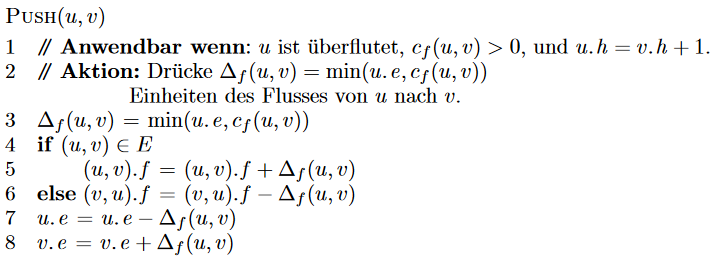
\includegraphics{../Grafiken/Push.png}
\end{adjustbox}
\end{frame}

\begin{frame}
\frametitle{Relabel-Operation}
\begin{adjustbox}{width = \textwidth}
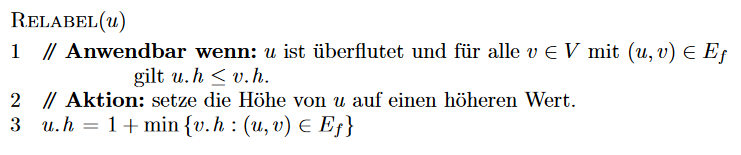
\includegraphics{../Grafiken/Relabel.png}
\end{adjustbox}
\end{frame}

\begin{frame}
\frametitle{generischer \pr -Algorithmus}
\centering
\begin{adjustbox}{width = 0.5\textwidth}
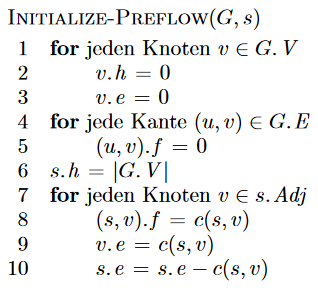
\includegraphics{../Grafiken/Init-Preflow.png}
\end{adjustbox}
\begin{adjustbox}{width = \textwidth}
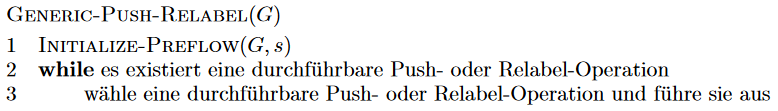
\includegraphics{../Grafiken/Generic-PR.png}
\end{adjustbox}
\end{frame}

\begin{frame}
\frametitle{\pr -Beispiel}
\begin{figure}
\centering
\begin{subfigure}{0.45\textwidth}
\begin{adjustbox}{width =\linewidth}
\begin{tikzpicture}
\Vertex[label=$s$]{s}
\Vertex[label=$v_1$, x=2, y=1]{1}
\Vertex[label=$v_2$, x=2, y=-1]{2}
\Vertex[label=$t$, x=4]{t}
\Edge[Direct, label=3](s)(1)
\Edge[Direct, label=4](s)(2)
\Edge[Direct, label=3](1)(2)
\Edge[Direct, label=1](1)(t)
\Edge[Direct, label=5](2)(t)
\end{tikzpicture}
\end{adjustbox}
\end{subfigure}
\begin{subfigure}{0.45\textwidth}
\begin{adjustbox}{width =\linewidth}
\begin{tikzpicture}
\draw[step=1cm,gray,very thin] (0,0) grid (5,5);
\draw (5,0) node[anchor=north west] {$u \in V$};
\draw[thick,->] (0,0) -- (0,5) node[anchor=south east] {$h(u)$};
\foreach \y in {0,1,2,3,4}
    \draw (1pt,\y cm) -- (-1pt,\y cm) node[anchor=east] {$\y$};

\Vertex[label=$s$, x=1, y=0]{s}
\Vertex[label=$v_1$, x=2, y=0]{1}
\Vertex[label=$v_2$, x=3, y=0]{2}
\Vertex[label=$t$, x=4, y=0]{t}

\draw (5,5.5) node[anchor=south west, text=red] {\large u.e};
\draw (1,5.5) node[anchor=south, text=red] {\large 0};
\draw (2,5.5) node[anchor=south, text=red] {\large 0};
\draw (3,5.5) node[anchor=south, text=red] {\large 0};
\draw (4,5.5) node[anchor=south, text=red] {\large 0};
\end{tikzpicture}
\end{adjustbox}
\end{subfigure}
\end{figure}
\note{Knotenhöhen und -überschüsse bereits initialisiert}
\note{Diagramm rechts erläutern: Knoten, Höhen und Überschüsse}
\end{frame}

\begin{frame}
\frametitle{\pr -Beispiel}
\begin{figure}
\centering
\begin{subfigure}{0.45\textwidth}
\begin{adjustbox}{width =\linewidth}
\begin{tikzpicture}
\Vertex[label=$s$]{s}
\Vertex[label=$v_1$, x=2, y=1, color=lime]{1}
\Vertex[label=$v_2$, x=2, y=-1]{2}
\Vertex[label=$t$, x=4]{t}
\Edge[Direct, label=3/3](s)(1)
\Edge[Direct, label=4/4](s)(2)
\Edge[Direct, label=3](1)(2)
\Edge[Direct, label=1](1)(t)
\Edge[Direct, label=5](2)(t)
\end{tikzpicture}
\end{adjustbox}
\end{subfigure}
\begin{subfigure}{0.45\textwidth}
\begin{adjustbox}{width =\linewidth}
\begin{tikzpicture}
\draw[step=1cm,gray,very thin] (0,0) grid (5,5);
\draw (5,0) node[anchor=north west] {$u \in V$};
\draw[thick,->] (0,0) -- (0,5) node[anchor=south east] {$h(u)$};
\foreach \y in {0,1,2,3,4}
    \draw (1pt,\y cm) -- (-1pt,\y cm) node[anchor=east] {$\y$};
\Vertex[label=$s$, x=1, y=4]{s}
\Vertex[label=$v_1$, x=2, y=0, color=lime]{1}
\Vertex[label=$v_2$, x=3, y=0]{2}
\Vertex[label=$t$, x=4, y=0]{t}
\draw (5,5.5) node[anchor=south west, text=red] {\large u.e};
\draw (1,5.5) node[anchor=south, text=red] {\large -7};
\draw (2,5.5) node[anchor=south, text=red] {\large 3};
\draw (3,5.5) node[anchor=south, text=red] {\large 4};
\draw (4,5.5) node[anchor=south, text=red] {\large 0};
\end{tikzpicture}
\end{adjustbox}
\end{subfigure}
\end{figure}
\note{"initialize preflow" abgeschlossen}
\note{in anderer Farbe der für die nächste Operation betrachtete Knoten (push nicht anwendbar, aber relabel -> auf t.h+1= v2.h+1 setzen)}
\end{frame}

\begin{frame}
\frametitle{\pr -Beispiel}
\begin{figure}
\centering
\begin{subfigure}{0.45\textwidth}
\begin{adjustbox}{width =\linewidth}
\begin{tikzpicture}
\Vertex[label=$s$]{s}
\Vertex[label=$v_1$, x=2, y=1, color=lime]{1}
\Vertex[label=$v_2$, x=2, y=-1]{2}
\Vertex[label=$t$, x=4]{t}
\Edge[Direct, label=3/3](s)(1)
\Edge[Direct, label=4/4](s)(2)
\Edge[Direct, label=3](1)(2)
\Edge[Direct, label=1, color=lime](1)(t)
\Edge[Direct, label=5](2)(t)
\end{tikzpicture}
\end{adjustbox}
\end{subfigure}
\begin{subfigure}{0.45\textwidth}
\begin{adjustbox}{width =\linewidth}
\begin{tikzpicture}
\draw[step=1cm,gray,very thin] (0,0) grid (5,5);
\draw (5,0) node[anchor=north west] {$u \in V$};
\draw[thick,->] (0,0) -- (0,5) node[anchor=south east] {$h(u)$};
\foreach \y in {0,1,2,3,4}
    \draw (1pt,\y cm) -- (-1pt,\y cm) node[anchor=east] {$\y$};
\Vertex[label=$s$, x=1, y=4]{s}
\Vertex[label=$v_1$, x=2, y=1, color=lime]{1}
\Vertex[label=$v_2$, x=3, y=0]{2}
\Vertex[label=$t$, x=4, y=0]{t}
\draw (5,5.5) node[anchor=south west, text=red] {\large u.e};
\draw (1,5.5) node[anchor=south, text=red] {\large -7};
\draw (2,5.5) node[anchor=south, text=red] {\large 3};
\draw (3,5.5) node[anchor=south, text=red] {\large 4};
\draw (4,5.5) node[anchor=south, text=red] {\large 0};
\end{tikzpicture}
\end{adjustbox}
\end{subfigure}
\end{figure}
\note{Fluss kann von v1 nach t (oder v2) gepusht werden.}
\note{pushe das Minimum von Kapazität der Restkante und Überschuss}
\end{frame}

\begin{frame}
\frametitle{\pr -Beispiel}
\begin{figure}
\centering
\begin{subfigure}{0.45\textwidth}
\begin{adjustbox}{width =\linewidth}
\begin{tikzpicture}
\Vertex[label=$s$]{s}
\Vertex[label=$v_1$, x=2, y=1, color=lime]{1}
\Vertex[label=$v_2$, x=2, y=-1]{2}
\Vertex[label=$t$, x=4]{t}
\Edge[Direct, label=3/3](s)(1)
\Edge[Direct, label=4/4](s)(2)
\Edge[Direct, label=3, color=lime](1)(2)
\Edge[Direct, label=1/1](1)(t)
\Edge[Direct, label=5](2)(t)
\end{tikzpicture}
\end{adjustbox}
\end{subfigure}
\begin{subfigure}{0.45\textwidth}
\begin{adjustbox}{width =\linewidth}
\begin{tikzpicture}
\draw[step=1cm,gray,very thin] (0,0) grid (5,5);
\draw (5,0) node[anchor=north west] {$u \in V$};
\draw[thick,->] (0,0) -- (0,5) node[anchor=south east] {$h(u)$};
\foreach \y in {0,1,2,3,4}
    \draw (1pt,\y cm) -- (-1pt,\y cm) node[anchor=east] {$\y$};
\Vertex[label=$s$, x=1, y=4]{s}
\Vertex[label=$v_1$, x=2, y=1, color=lime]{1}
\Vertex[label=$v_2$, x=3, y=0]{2}
\Vertex[label=$t$, x=4, y=0]{t}
\draw (5,5.5) node[anchor=south west, text=red] {\large u.e};
\draw (1,5.5) node[anchor=south, text=red] {\large -7};
\draw (2,5.5) node[anchor=south, text=red] {\large 2};
\draw (3,5.5) node[anchor=south, text=red] {\large 4};
\draw (4,5.5) node[anchor=south, text=red] {\large 1};
\end{tikzpicture}
\end{adjustbox}
\end{subfigure}
\end{figure}
\note{weitere push-Operation verfügbar}
\end{frame}

\begin{frame}
\frametitle{\pr -Beispiel}
\begin{figure}
\centering
\begin{subfigure}{0.45\textwidth}
\begin{adjustbox}{width =\linewidth}
\begin{tikzpicture}
\Vertex[label=$s$]{s}
\Vertex[label=$v_1$, x=2, y=1]{1}
\Vertex[label=$v_2$, x=2, y=-1, color=lime]{2}
\Vertex[label=$t$, x=4]{t}
\Edge[Direct, label=3/3](s)(1)
\Edge[Direct, label=4/4](s)(2)
\Edge[Direct, label=2/3](1)(2)
\Edge[Direct, label=1/1](1)(t)
\Edge[Direct, label=5](2)(t)
\end{tikzpicture}
\end{adjustbox}
\end{subfigure}
\begin{subfigure}{0.45\textwidth}
\begin{adjustbox}{width =\linewidth}
\begin{tikzpicture}
\draw[step=1cm,gray,very thin] (0,0) grid (5,5);
\draw (5,0) node[anchor=north west] {$u \in V$};
\draw[thick,->] (0,0) -- (0,5) node[anchor=south east] {$h(u)$};
\foreach \y in {0,1,2,3,4}
    \draw (1pt,\y cm) -- (-1pt,\y cm) node[anchor=east] {$\y$};
\Vertex[label=$s$, x=1, y=4]{s}
\Vertex[label=$v_1$, x=2, y=1]{1}
\Vertex[label=$v_2$, x=3, y=0, color=lime]{2}
\Vertex[label=$t$, x=4, y=0]{t}
\draw (5,5.5) node[anchor=south west, text=red] {\large u.e};
\draw (1,5.5) node[anchor=south, text=red] {\large -7};
\draw (2,5.5) node[anchor=south, text=red] {\large 0};
\draw (3,5.5) node[anchor=south, text=red] {\large 6};
\draw (4,5.5) node[anchor=south, text=red] {\large 1};
\end{tikzpicture}
\end{adjustbox}
\end{subfigure}
\end{figure}
\note{relabel v2 auf t.h + 1}
\end{frame}

\begin{frame}
\frametitle{\pr -Beispiel}
\begin{figure}
\centering
\begin{subfigure}{0.45\textwidth}
\begin{adjustbox}{width =\linewidth}
\begin{tikzpicture}
\Vertex[label=$s$]{s}
\Vertex[label=$v_1$, x=2, y=1]{1}
\Vertex[label=$v_2$, x=2, y=-1, color=lime]{2}
\Vertex[label=$t$, x=4]{t}
\Edge[Direct, label=3/3](s)(1)
\Edge[Direct, label=4/4](s)(2)
\Edge[Direct, label=2/3](1)(2)
\Edge[Direct, label=1/1](1)(t)
\Edge[Direct, label=5, color=lime](2)(t)
\end{tikzpicture}
\end{adjustbox}
\end{subfigure}
\begin{subfigure}{0.45\textwidth}
\begin{adjustbox}{width =\linewidth}
\begin{tikzpicture}
\draw[step=1cm,gray,very thin] (0,0) grid (5,5);
\draw (5,0) node[anchor=north west] {$u \in V$};
\draw[thick,->] (0,0) -- (0,5) node[anchor=south east] {$h(u)$};
\foreach \y in {0,1,2,3,4}
    \draw (1pt,\y cm) -- (-1pt,\y cm) node[anchor=east] {$\y$};
\Vertex[label=$s$, x=1, y=4]{s}
\Vertex[label=$v_1$, x=2, y=1]{1}
\Vertex[label=$v_2$, x=3, y=1, color=lime]{2}
\Vertex[label=$t$, x=4, y=0]{t}
\draw (5,5.5) node[anchor=south west, text=red] {\large u.e};
\draw (1,5.5) node[anchor=south, text=red] {\large -7};
\draw (2,5.5) node[anchor=south, text=red] {\large 0};
\draw (3,5.5) node[anchor=south, text=red] {\large 6};
\draw (4,5.5) node[anchor=south, text=red] {\large 1};
\end{tikzpicture}
\end{adjustbox}
\end{subfigure}
\end{figure}
\note{push 5}
\end{frame}

\begin{frame}
\frametitle{\pr -Beispiel}
\begin{figure}
\centering
\begin{subfigure}{0.45\textwidth}
\begin{adjustbox}{width =\linewidth}
\begin{tikzpicture}
\Vertex[label=$s$]{s}
\Vertex[label=$v_1$, x=2, y=1]{1}
\Vertex[label=$v_2$, x=2, y=-1, color=lime]{2}
\Vertex[label=$t$, x=4]{t}
\Edge[Direct, label=3/3](s)(1)
\Edge[Direct, label=4/4](s)(2)
\Edge[Direct, label=2/3](1)(2)
\Edge[Direct, label=1/1](1)(t)
\Edge[Direct, label=5/5](2)(t)
\end{tikzpicture}
\end{adjustbox}
\end{subfigure}
\begin{subfigure}{0.45\textwidth}
\begin{adjustbox}{width =\linewidth}
\begin{tikzpicture}
\draw[step=1cm,gray,very thin] (0,0) grid (5,5);
\draw (5,0) node[anchor=north west] {$u \in V$};
\draw[thick,->] (0,0) -- (0,5) node[anchor=south east] {$h(u)$};
\foreach \y in {0,1,2,3,4}
    \draw (1pt,\y cm) -- (-1pt,\y cm) node[anchor=east] {$\y$};
\Vertex[label=$s$, x=1, y=4]{s}
\Vertex[label=$v_1$, x=2, y=1]{1}
\Vertex[label=$v_2$, x=3, y=1, color=lime]{2}
\Vertex[label=$t$, x=4, y=0]{t}
\draw (5,5.5) node[anchor=south west, text=red] {\large u.e};
\draw (1,5.5) node[anchor=south, text=red] {\large -7};
\draw (2,5.5) node[anchor=south, text=red] {\large 0};
\draw (3,5.5) node[anchor=south, text=red] {\large 1};
\draw (4,5.5) node[anchor=south, text=red] {\large 6};
\end{tikzpicture}
\end{adjustbox}
\end{subfigure}
\end{figure}
\note{relabel v2}
\end{frame}

\begin{frame}
\frametitle{\pr -Beispiel}
\begin{figure}
\centering
\begin{subfigure}{0.45\textwidth}
\begin{adjustbox}{width =\linewidth}
\begin{tikzpicture}
\Vertex[label=$s$]{s}
\Vertex[label=$v_1$, x=2, y=1]{1}
\Vertex[label=$v_2$, x=2, y=-1, color=lime]{2}
\Vertex[label=$t$, x=4]{t}
\Edge[Direct, label=3/3](s)(1)
\Edge[Direct, label=4/4](s)(2)
\Edge[Direct, label=2/3, color=lime](1)(2)
\Edge[Direct, label=1/1](1)(t)
\Edge[Direct, label=5/5](2)(t)
\end{tikzpicture}
\end{adjustbox}
\end{subfigure}
\begin{subfigure}{0.45\textwidth}
\begin{adjustbox}{width =\linewidth}
\begin{tikzpicture}
\draw[step=1cm,gray,very thin] (0,0) grid (5,5);
\draw (5,0) node[anchor=north west] {$u \in V$};
\draw[thick,->] (0,0) -- (0,5) node[anchor=south east] {$h(u)$};
\foreach \y in {0,1,2,3,4}
    \draw (1pt,\y cm) -- (-1pt,\y cm) node[anchor=east] {$\y$};
\Vertex[label=$s$, x=1, y=4]{s}
\Vertex[label=$v_1$, x=2, y=1]{1}
\Vertex[label=$v_2$, x=3, y=2, color=lime]{2}
\Vertex[label=$t$, x=4, y=0]{t}
\draw (5,5.5) node[anchor=south west, text=red] {\large u.e};
\draw (1,5.5) node[anchor=south, text=red] {\large -7};
\draw (2,5.5) node[anchor=south, text=red] {\large 0};
\draw (3,5.5) node[anchor=south, text=red] {\large 1};
\draw (4,5.5) node[anchor=south, text=red] {\large 6};
\end{tikzpicture}
\end{adjustbox}
\end{subfigure}
\end{figure}
\note{push 1 to v1 (Kapazitäten des Restnetzwerks!)}
\end{frame}

\begin{frame}
\frametitle{\pr -Beispiel}
\begin{figure}
\centering
\begin{subfigure}{0.45\textwidth}
\begin{adjustbox}{width =\linewidth}
\begin{tikzpicture}
\Vertex[label=$s$]{s}
\Vertex[label=$v_1$, x=2, y=1, color=lime]{1}
\Vertex[label=$v_2$, x=2, y=-1]{2}
\Vertex[label=$t$, x=4]{t}
\Edge[Direct, label=3/3](s)(1)
\Edge[Direct, label=4/4](s)(2)
\Edge[Direct, label=1/3](1)(2)
\Edge[Direct, label=1/1](1)(t)
\Edge[Direct, label=5/5](2)(t)
\end{tikzpicture}
\end{adjustbox}
\end{subfigure}
\begin{subfigure}{0.45\textwidth}
\begin{adjustbox}{width =\linewidth}
\begin{tikzpicture}
\draw[step=1cm,gray,very thin] (0,0) grid (5,5);
\draw (5,0) node[anchor=north west] {$u \in V$};
\draw[thick,->] (0,0) -- (0,5) node[anchor=south east] {$h(u)$};
\foreach \y in {0,1,2,3,4}
    \draw (1pt,\y cm) -- (-1pt,\y cm) node[anchor=east] {$\y$};
\Vertex[label=$s$, x=1, y=4]{s}
\Vertex[label=$v_1$, x=2, y=1, color=lime]{1}
\Vertex[label=$v_2$, x=3, y=2]{2}
\Vertex[label=$t$, x=4, y=0]{t}
\draw (5,5.5) node[anchor=south west, text=red] {\large u.e};
\draw (1,5.5) node[anchor=south, text=red] {\large -7};
\draw (2,5.5) node[anchor=south, text=red] {\large 1};
\draw (3,5.5) node[anchor=south, text=red] {\large 0};
\draw (4,5.5) node[anchor=south, text=red] {\large 6};
\end{tikzpicture}
\end{adjustbox}
\end{subfigure}
\end{figure}
\note{"Hochschaukeln" -> Zusammenfassen von Relabel v1 und push 1 to v2}
\end{frame}

\begin{frame}
\frametitle{\pr -Beispiel}
\begin{figure}
\centering
\begin{subfigure}{0.45\textwidth}
\begin{adjustbox}{width =\linewidth}
\begin{tikzpicture}
\Vertex[label=$s$]{s}
\Vertex[label=$v_1$, x=2, y=1]{1}
\Vertex[label=$v_2$, x=2, y=-1, color=lime]{2}
\Vertex[label=$t$, x=4]{t}
\Edge[Direct, label=3/3](s)(1)
\Edge[Direct, label=4/4](s)(2)
\Edge[Direct, label=2/3, color=lime](1)(2)
\Edge[Direct, label=1/1](1)(t)
\Edge[Direct, label=5/5](2)(t)
\end{tikzpicture}
\end{adjustbox}
\end{subfigure}
\begin{subfigure}{0.45\textwidth}
\begin{adjustbox}{width =\linewidth}
\begin{tikzpicture}
\draw[step=1cm,gray,very thin] (0,0) grid (5,5);
\draw (5,0) node[anchor=north west] {$u \in V$};
\draw[thick,->] (0,0) -- (0,5) node[anchor=south east] {$h(u)$};
\foreach \y in {0,1,2,3,4}
    \draw (1pt,\y cm) -- (-1pt,\y cm) node[anchor=east] {$\y$};
\Vertex[label=$s$, x=1, y=4]{s}
\Vertex[label=$v_1$, x=2, y=3]{1}
\Vertex[label=$v_2$, x=3, y=2, color=lime]{2}
\Vertex[label=$t$, x=4, y=0]{t}
\draw (5,5.5) node[anchor=south west, text=red] {\large u.e};
\draw (1,5.5) node[anchor=south, text=red] {\large -7};
\draw (2,5.5) node[anchor=south, text=red] {\large 0};
\draw (3,5.5) node[anchor=south, text=red] {\large 1};
\draw (4,5.5) node[anchor=south, text=red] {\large 6};
\end{tikzpicture}
\end{adjustbox}
\end{subfigure}
\end{figure}
\note{push 1 to v1 (Kapazitäten des Restnetzwerks!)}
\end{frame}

\begin{frame}
\frametitle{\pr -Beispiel}
\begin{figure}
\centering
\begin{subfigure}{0.45\textwidth}
\begin{adjustbox}{width =\linewidth}
\begin{tikzpicture}
\Vertex[label=$s$]{s}
\Vertex[label=$v_1$, x=2, y=1, color=lime]{1}
\Vertex[label=$v_2$, x=2, y=-1]{2}
\Vertex[label=$t$, x=4]{t}
\Edge[Direct, label=3/3](s)(1)
\Edge[Direct, label=4/4](s)(2)
\Edge[Direct, label=1/3](1)(2)
\Edge[Direct, label=1/1](1)(t)
\Edge[Direct, label=5/5](2)(t)
\end{tikzpicture}
\end{adjustbox}
\end{subfigure}
\begin{subfigure}{0.45\textwidth}
\begin{adjustbox}{width =\linewidth}
\begin{tikzpicture}
\draw[step=1cm,gray,very thin] (0,0) grid (5,5);
\draw (5,0) node[anchor=north west] {$u \in V$};
\draw[thick,->] (0,0) -- (0,5) node[anchor=south east] {$h(u)$};
\foreach \y in {0,1,2,3,4}
    \draw (1pt,\y cm) -- (-1pt,\y cm) node[anchor=east] {$\y$};
\Vertex[label=$s$, x=1, y=4]{s}
\Vertex[label=$v_1$, x=2, y=3, color=lime]{1}
\Vertex[label=$v_2$, x=3, y=4]{2}
\Vertex[label=$t$, x=4, y=0]{t}
\draw (5,5.5) node[anchor=south west, text=red] {\large u.e};
\draw (1,5.5) node[anchor=south, text=red] {\large -7};
\draw (2,5.5) node[anchor=south, text=red] {\large 1};
\draw (3,5.5) node[anchor=south, text=red] {\large 0};
\draw (4,5.5) node[anchor=south, text=red] {\large 6};
\end{tikzpicture}
\end{adjustbox}
\end{subfigure}
\end{figure}
\end{frame}

\begin{frame}
\frametitle{\pr -Beispiel}
\begin{figure}
\centering
\begin{subfigure}{0.45\textwidth}
\begin{adjustbox}{width =\linewidth}
\begin{tikzpicture}
\Vertex[label=$s$]{s}
\Vertex[label=$v_1$, x=2, y=1, color=lime]{1}
\Vertex[label=$v_2$, x=2, y=-1]{2}
\Vertex[label=$t$, x=4]{t}
\Edge[Direct, label=3/3, color=lime](s)(1)
\Edge[Direct, label=4/4](s)(2)
\Edge[Direct, label=1/3](1)(2)
\Edge[Direct, label=1/1](1)(t)
\Edge[Direct, label=5/5](2)(t)
\end{tikzpicture}
\end{adjustbox}
\end{subfigure}
\begin{subfigure}{0.45\textwidth}
\begin{adjustbox}{width =\linewidth}
\begin{tikzpicture}
\draw[step=1cm,gray,very thin] (0,0) grid (5,5);
\draw (5,0) node[anchor=north west] {$u \in V$};
\draw[thick,->] (0,0) -- (0,5) node[anchor=south east] {$h(u)$};
\foreach \y in {0,1,2,3,4}
    \draw (1pt,\y cm) -- (-1pt,\y cm) node[anchor=east] {$\y$};
\Vertex[label=$s$, x=1, y=4]{s}
\Vertex[label=$v_1$, x=2, y=5, color=lime]{1}
\Vertex[label=$v_2$, x=3, y=4]{2}
\Vertex[label=$t$, x=4, y=0]{t}
\draw (5,5.5) node[anchor=south west, text=red] {\large u.e};
\draw (1,5.5) node[anchor=south, text=red] {\large -7};
\draw (2,5.5) node[anchor=south, text=red] {\large 1};
\draw (3,5.5) node[anchor=south, text=red] {\large 0};
\draw (4,5.5) node[anchor=south, text=red] {\large 6};
\end{tikzpicture}
\end{adjustbox}
\end{subfigure}
\end{figure}
\note{durch Erhöhung über $\lvert V\rvert$ wieder pushen in Quelle möglich}
\end{frame}

\begin{frame}
\frametitle{\pr -Beispiel}
\begin{figure}
\centering
\begin{subfigure}{0.45\textwidth}
\begin{adjustbox}{width =\linewidth}
\begin{tikzpicture}
\Vertex[label=$s$]{s}
\Vertex[label=$v_1$, x=2, y=1]{1}
\Vertex[label=$v_2$, x=2, y=-1]{2}
\Vertex[label=$t$, x=4]{t}
\Edge[Direct, label=2/3](s)(1)
\Edge[Direct, label=4/4](s)(2)
\Edge[Direct, label=1/3](1)(2)
\Edge[Direct, label=1/1](1)(t)
\Edge[Direct, label=5/5](2)(t)
\end{tikzpicture}
\end{adjustbox}
\end{subfigure}
\begin{subfigure}{0.45\textwidth}
\begin{adjustbox}{width =\linewidth}
\begin{tikzpicture}
\draw[step=1cm,gray,very thin] (0,0) grid (5,5);
\draw (5,0) node[anchor=north west] {$u \in V$};
\draw[thick,->] (0,0) -- (0,5) node[anchor=south east] {$h(u)$};
\foreach \y in {0,1,2,3,4}
    \draw (1pt,\y cm) -- (-1pt,\y cm) node[anchor=east] {$\y$};
\Vertex[label=$s$, x=1, y=4]{s}
\Vertex[label=$v_1$, x=2, y=5]{1}
\Vertex[label=$v_2$, x=3, y=4]{2}
\Vertex[label=$t$, x=4, y=0]{t}
\draw (5,5.5) node[anchor=south west, text=red] {\large u.e};
\draw (1,5.5) node[anchor=south, text=red] {\large -6};
\draw (2,5.5) node[anchor=south, text=red] {\large 0};
\draw (3,5.5) node[anchor=south, text=red] {\large 0};
\draw (4,5.5) node[anchor=south, text=red] {\large 6};
\end{tikzpicture}
\end{adjustbox}
\end{subfigure}
\end{figure}
\note{keine Operationen mehr möglich -> f ist maximaler Fluss}
\note{Operationen im Beispiel bereits in günstiger Reihenfolge gewählt -> Verbesserungen}
\end{frame}

\begin{frame}
\frametitle{\pr -Analyse}
\begin{itemize}
\item Vorfluss $f$ ist bei Terminierung ein Fluss.
\note{Beweis über mehrere Beobachtungen zur Höhenfunktion und eine Schleifeninvariante}
\note{Terminierung über Abschätzung der benötigten Operationen}
\item insgesamt $\mathcal{O}(V^2 \cdot E)$
\item Verbesserung: Relabel-to-Front-Algorithmus
\note{geschickte Wahl der Datenstruktur und der ausgeführten Operationen}
\item $\mathcal{O}(V^3)$
\end{itemize}
\end{frame}

\begin{frame}
\frametitle{Literatur}
\bibliography{../../references}
\bibliographystyle{ieeetr}
\end{frame}

\end{document}
